\section{Equazioni differenziali}
\subsection{Definizioni}
Un'equazione differenziale è una relazione tra una funzione incognita $y=y(t)$ e alcune sue derivate.\newline
\newline
Si dice \textbf{equazione differenziale di ordine} $n$ un equazione del tipo:
\[
    F(t, y(t), y'(t), y''(t), \dots, y^{(n)}(t)) = 0 \;\;\;\;\;\;\;(t \in I)
\]
dove $y(t)$ è la funzione incognita.\newline
\newline
Si dirà \textbf{soluzione}, o (curva) integrale, di un equazione differenziale, nell'intervallo $I$, una funzione $\phi(t)$, definita almeno in $I$ (ma in generale può essere definita in $J \subseteq I$) e a valori reali per cui risulti
\[
    F(t, \phi(t), \phi'(t), \phi''(t), \dots, \phi^{(n)}(t))= 0 \;\;\;\;\;\;\;\; \;\forall\;t \in J
\]
\ \newline
\newline
Diremo che un'equazione differenziale è in \textbf{forma normale} se è possibile esplicitare la derivata di ordine massimo in funzione di tutte le derivate di ordine inferiore:
\[
    y^{(n)}(t) = g(t,y(t),y'(t),y''(t), \dots, y^{(n-1)}(t)) \;\;\;\;\;\;\;(t \in I)
\]
\ \newline
\newline
\textbf{Problema di Cauchy}:
Data un'equazione in forma normale
\[
    y^{(n)}(t) = g(t,y(t),y'(t),y''(t), \dots, y^{(n-1)}(t)) \;\;\;\;\;\;\;(t \in I)
\]
a essa vengono associate $n$ delle condizioni
\[
    y(t_0) = y_0 \;\;\;\;\; y'(t_0)=y_1 \;\;\;\;\;\dots \;\;\;\;\;y^{(n-1)}(t_0) = y_{n-1}
\]
dove $t_0$ rappresenta l'istante iniziale e $y_0,\dots,y_{n-1}$ rappresentano lo stato. Risolvere un problema di Cauchy significa riuscire a prevedere come si comproterà la $y(t)$ (stato del sistema) negli istanti futuri $t>t_0$. Per risolvere un problema di Cauchy si intende sempre che bisogna trovare come soluzione una funzione:
\begin{itemize}
    \item definita su un intervallo $I$, contenente il punto $t_0$;
    \item derivabile in tutto $I$ e che soddisfa l'equazione in tutto $I$.
\end{itemize}
\ \newline
Chiameremo \textbf{integrale generale} di un'equazione differenziale l'insieme di tutte le sue infinite soluzioni; chiameremo invece \textbf{integrale particolare} una sua soluzione che soddisfa particolari proprietà quali, ad esempio, quelle imposte dal problema di Cauchy.\newline
\newline
L'integrale generale è ricavabile dall'equazione in forma normale con vari metodi che vediamo più avanti, mentre le varie condizioni permettono di ricavare un integrale particolare.
\subsection{Esistenza e unicità}
In questo paragrafo studiamo l'esistena e l'unicità per il problema di Cauchy nel caso di equazioni differenziali del prim'oridne in forma normale. Se un equazione fosse di ordine superiore, ad esempio del second'ordine $y'' = f(t,y,y')$, con un semplice trucco potremmo ricondurci a un sistema del prim'ordine: basta porre $z = y'$ e la precedente equazione del second'ordine si traduce nelle due seguenti equazioni del prim'ordine: $y'=z$ e $z' = f(t,y,z)$,  dove l'incognita è adesso il vettore $(y,z)$.\newline
\newline
\textbf{teor.} \textbf{Teorema di Peano}:\newline
Sia $\Omega \subset \mathbb{R}^2$ un aperto e sia $(t_0, y_0) \in \Omega$. Se $f \in C^0 (\Omega)$ allora esiste una soluzione del problema di Cauchy:
\[
    \begin{cases}
        y' = f(t,y)\\ y(t_0) = y_0
    \end{cases}
\]
\ \newline
\textbf{teor.} \textbf{Teorema di Cauchy}:\newline
Sia $\Omega \subset \mathbb{R}^2$ un aperto e sia $(t_0, y_0) \in \Omega$. Se $f,f_y \in C^0(\Omega)$, allora esiste un'unica soluzione del problema di Cauchy:
\[
    \begin{cases}
        y' = f(t,y)\\ y(t_0) = y_0
    \end{cases}
\]
\subsection{Equazioni del primo ordine}
Analiziamo ora vari metodi per risolvere il problema di Cauchy per equazioni del prim'ordine:
\[
    \begin{cases}
        y' = f(t,y)\\ y(t_0) = y_0
    \end{cases}
\]
\subsubsection{Equazioni a variabili separabili}
Un'equazione differenziale del tipo
\[
    y' = f(t)g(y)
\]
si dice \textbf{equazione a variabili separabili}.\newline
\newline
Dai teoremi di Cauchy e di Peano ricaviamo il seguente corollario:\newline
Siamo $t_0,y_0 \in \mathbb{R}$ e sia $f$ continua in un intorno di $t_0$:
\begin{itemize}
    \item Se $g$ è continua in un intorno di $y_0$, allora il problema di Cauchy $y(t_0) = y_0$ per l'equazione a variabili separabili $y'=f(t)g(y)$ ammette una soluzione.
    \item Se $g$ è di classe $C^1$ in un intorno di $y_0$, allora il problema di Cauchy $y(t_0) = y_0$ per l'equazione a variabil iseparabili $y'=f(t) g(y)$ ammette una e una sola soluzione.
\end{itemize}
\ \newline
Come prima cosa, osserviamo che se esiste $\bar{y} \in \mathbb{R}$ tale che $g(\bar{y}) = 0$ allora $y(t) \equiv \bar{y}$ è una soluzione costante dell'equazione a variabili separabili; pertanto, se all'equazione a variabili separabili associamo il problema di cauchy $y(t_0) = \bar{y}$ abbiamo già trovato una soluzione (naturalmente se $g$ è solo continua potrebbero essercene altre). Ma supponiamo di considerare un problema di cauchy $y(t_0) = y_0$ con $g(y_0) \neq 0$, in modo da poter dividere l'intera equazione a variabili separabili per $g(y)$ (almeno in un intorno di $y_0$). Usando la notazione $y' = \frac{dy}{dt}$, i semplici passaggi per risolvere l'equazione a variabil iseparabili $y' = f(t) g(y)$ sono i seguenti:
\[
    \frac{dy}{dt} = f(t) g(y) \Longrightarrow \frac{dy}{g(y)} = f(t) dt \Longrightarrow \int \frac{1}{g(y)}dy = \int f(t) dt
\]
A questo punto, una volta risolti gli integrali, è sufficiente esprimere $y$ in funzione di tutto il resto. Notiamo che gli integrali fanno comparire una costante arbitraria che verrà determinata risolvendo il problema di Cauchy.
\newline
\newline
\textbf{Procedimento per risolvere equazioni a variabili separabili}:
\begin{itemize}
    \item stabilire se $f,g \in C^0$ o se $g \in C^1$;
    \item risolvere l'equazione $g(\bar{y}) = 0$;
    \item tutte le soluzioni di questa equazione rappresentano soluzioni costanti;
    \item se $g \notin C^1$ ci potrebbe essere un pennello di Peano che si stacca dalla soluzione costante;
    \item se $g \in C^1$ c'è unicità e le soluzioni costanti rappresentano dei "limiti invalicabili" per le altre soluzioni;
    \item risolvere il problema di Cauchy.
\end{itemize}




Le equazioni a variabili separabili sono equazioni del tipo
\[
    y' =a(t) b(y)
\]
con $a$ continua in $I \subset \mathbb{R}$ e b continua in $J \subset \mathbb{R}$.\newline
Per risolverle notiamo che per tutte le $\bar{y}_0$ per cui $b(\bar{y}_0) = 0$, primo e secondo membro si annullano.\newline
Prendendo in considerazione, invece, tutte le $\bar{y}_1$ per cui $b(\bar{y}_1) \neq 0$, otteniamo:
\[
    \int \frac{dy}{b(y)} = \int a(t) dt +c 
\]
Quindi se $B(y)$ è una primitiva di $\frac{1}{b(y)}$ e $A(t)$ è una primitiva di $a(t)$, otteniamo:
\[
    B(y) = A(t) + c
\]
e se si può ottenere la funzione inversa di $B$ possiamo scrivere:
\[
    y = B^{-1}(A(t) + c)
\]
\[
    y = F(t,c)
\]
\textbf{teor.} Problema di Cauchy per un'equazione a variabili separabili.\newline
Si consideri il problema di Cauchy:
\[
    \begin{cases}
        y' = a(t) b(y)&\\
        y(t_0) = y_0&
    \end{cases}
\]
Dove $a$ è continua in un intorno $I$ di $t_0$ e $b$ è continua in un intonro $J$ di $t_0$. Allora essite un intorno $t_0$ $I' \subset I$ e una funzione $y \in C^1(I')$ soluzione del problema.\newline
Se inoltre $b \in C^1(J)$, allora tale soluzione è unica.
\subsubsection{Equazioni lineari}
Sono equazioni la cui forma normale è
\[
    y'(t) + a(t)y(t) = f(t)
\]
e viene chiama equazione completa.\newline
Se $f = 0$ l'equazione si dice omogenea.
\[
    z'(t) + a(t)z(t) = 0
\]
\textbf{teor.} L'integrale generale dell'equazione completa si ottiene aggiungengo all'integrale generale dell'omogenea una soluzione particolare della completa.\newline
\textbf{Soluzione dell'equazione omogenea}
\[
    z(t) = c e^{-\int a(t) dt}
\]
\textbf{Ricerca di una soluzione particolare dell'equazione completa}\newline
Se una soluzione particolare non si riesce a trovare facilmente, si può usare il seguente metodo, detto di variazione della costante
\[
    \bar{y}(t) = c(t)e^{-A(t)}
\]
Dove per $A(t)$ si intende una primitiva di $a(t)$ (essendo una primitiva qualunque, si può omettere la $c$).\newline
Sostituendo $\bar{y}$ nella forma completa otteniamo l'integrale generale della forma completa:
\[
    y(t) = ce^{-A(t)} + e^{-A(t)}\int f(t)e^{A(t)}dt
\]
\textbf{oss.} Nella primitiva $A(t)$ e nell'integrale $\int f(t)e^{A(t)}dt$ non c'è bisogno di aggiungere la solita costante di integrazione arbitraria.\newline
\newline
\textbf{Soluzione del problema di Cauchy}\newline
La soluzione
\[
    y(t) = ce^{-A(t)} + e^{-A(t)}\int f(t)e^{A(t)}dt
\]
sarà determinata da una condizione iniziale
\[
    y(t_0) = y_0
\]
scegliendo la primitiva $A(t)$ tale che $A(t_0) = 0$ (cioè $A(t) = \int_{t_0}^{t}a(s)ds$), sarà
\[
    y(t) = ce^{-A(t)} + e^{-A(t)} \int_{t_0}^{t} f(s)e^{A(s)}ds
\]
\textbf{teor.} Problema di Cauchy per un equazione lineare del prim'ordine.\newline
Siano $a, f$ funzioni continue in un intervallo $I$ contenente $t_0$. Allora, per ogni $y_0 \in \mathbb{R}$ il problema di Cauchy
\[
    \begin{cases}
        y'(t) + a(t)y(t)= f(t)\\
        y(t_0) = y_0
    \end{cases}
\]
ha una e una sola soluzione $y \in C^1(I)$ e tale soluzione è
\[
    y(t) = ce^{-A(t)} + e^{-A(t)} \int_{t_0}^{t} f(s)e^{A(s)}ds
\]
\subsubsection{Note sugli esercizi}
Per trovare il massimo intervallo della soluzione bisogna prendere un intervallo contenente il punto $t_0$, per cui la soluzione e la funzione di partenza siano continue e definite (si può anche prolungare per continuità).
\subsubsection{Equazione di Bernoulli}
Un equazion differenziale si dice di \textbf{Bernoulli} se si può scrivere nella forma
\[
    y' = a(t)y + b(t) y^\alpha
\]
osserviamo subito che se $\alpha=0$ o $\alpha = 1$ l'equazione è lineare. Se poi $\alpha$ fosse irrazionale o razionale con denominatore pari, non avrebbe senso definire $y^\alpha$ per $y < 0$. Infine, se $\alpha < 0$ non ha senso $y^\alpha$ per $y=0$.\newline
\newline
Per evitare complicazioni ci occuperemo solo di soluzioni non negativa ($y \geq 0$).\newline
\newline
\textbf{teor.} Siano $t_0 \in \mathbb{R}$, $y_0 \geq 0$ e siano $a,b \in C^0$ in un intorno di $t_0$. Allora il problema di Cauchy $y(t_0) = y_0$ per un equazione di Bernoulli ammette una e una sola soluzione nei seguenti casi:
\[
    \alpha> 1 \;\;\;\;\; y_0 \geq 0
\]
\[
    0< \alpha< 1 \;\;\;\;\;y_0 > 0
\]
\[
    \alpha<0 \;\;\;\;\;y_0 > 0
\]
Se $\alpha > 0$ l'equazione di bernoulli ammette anche la soluzione nulla $y=0$, pertanto se  $\alpha > 1$ e $y_0 = 0$, il problema di Cauchy ammette solo la soluzione nulla.\newline
Nel caso $y_0 = 0$ e $0<\alpha < 1$, è garantita l'esistenza di una soluzione per il problema di Cauchy $y(t_0) = 0$ ma non ne è assicurata l'unicità (potrebbe crearsi un pannello di Peano).\newline
Se $y_0 > 0$ la soluzione rimarrà strettamente positiva per $\alpha > 1$, potrenne agganciarsi alla soluzione $y= 0$ con un pannello di peano se $0< \alpha<1$, potrebbe tendere a $0$ con tangente verticale se $\alpha<0$ (in quest'ultimo caso, bisogna verificare il comportamento della funzione $b(t)$ che, annullandosi, potrebbe verificare l'infinito di $y^\alpha$).\newline
\newline
Risolvere un equazione di Bernoulli:\newline
Si divide l'equazione per $y^\alpha$ e si ottiene $y^{-\alpha} y' = a(t) y^{1-\alpha} + b(t)$.\newline
Si pone $z(t) = y(t)^{1-\alpha}$ e si ottiene $z' = (1-\alpha)a(t)z + (1-\alpha) b(t)$, che è un'equazione lineare e quindi possiamo risolvere con i soliti metodi. Una volta trovata la soluzione $z(t)$ (che sarà $\geq 0$ o $>0$ a seconda dei valori di $\alpha$), si determina $y(t) = z(t)^{\frac{1}{1-\alpha}}$\newline
\subsubsection{Prolungamento delle soluzioni}
\subsection{Equazioni lineari del secondo ordine}
\subsubsection{Spazi di funzioni}
Sia $I$ un intervallo e consideriamo l'insieme $\mathbb{F}$ di tutte le funzioni definite in $I$, a valori reali. Con le operazioni naturali di somma di due funzioni e prodotto per uno scalare:
\[
    (f+g)(x) = f(x) + g(x)
\]
\[
    (\lambda f)(x) = \lambda f()
\]
$\mathbb{F}$ risulta essere uno spazio vettoriale. \newline
\newline
\textbf{def.} definiamo $C^n(I)$ lo spazio delle funzioni dotate di derivata $n$-essima continua.
\subsubsection{Generalità sulle equazioni lineari. Problema di Cauchy}
Un equazione differenziale del secondo ordine si dice lineare se è del tipo
\[
    a_2(t) y'' + a_1(t) y' +a_0(t) y = g(t)
\]
dove le funzioni $a_i$ e il termine noto $g$ sono funzioni continue in un certo intervallo $I$.\newline
Se il termine noto è nulla l'equazione si dice omogenea, altrimenti si dice completa.\newline
Se i coefficienti $a_i$ sono costanti, l'equazione si dirà a coefficienti costanti, altrimenti a coefficienti variabili.\newline
Se $a_2 = 1$ l'equazione si dirà in forma normale (se in un equazione il coefficiente $a_2$ non si annulla mai possiamo riscrivere l'equazione in fomra normale dividendo per questo).\newline
\newline
Nella soluzione si avranno sempre due coefficienti $c_1$ e $c_2$, per selezionare una soluzione particolare avremo bisogno di due condizioni iniziali:
\[
    \begin{cases}
        y(t_0) = y_0&\\
        y'(t_0) = y_1
    \end{cases}
\]
che insieme all'equazione iniziale prenderà il nome di problema di Cauchy.\newline
\newline
\textbf{teor.} (per funzioni del secondo ordine in forma normale)\newline
Se $a, b, f$ sono funzioni continue in un intervallo $I$ contenente il punto $t_0$, per ogni $y_0, y_1 \in \mathbb{R}$ il problema di Cauchy
\[
    \begin{cases}
        y'' + a(t) y' + b(t) y = f(t)\\
        y(t_0) = y_0\\
        y'(t_0) = y_1
    \end{cases}
\]
ha una e una sola soluzione $y \in C^2(I)$.\newline
Tale soluzione è individuata imponendo le condizioni iniziali nell'espressione che assegna l'integrale generale dell'equazione.
\subsubsection{La struttura dell'integrale generale}
\textbf{teor.} Struttura dell'integrale generale dell'equazione lineare completa \newline
a. $\;\;\;$ L'insieme delle soluzioni dell'equazione omogenea $Lz = 0 $ con $L:C^2(I)\rightarrow C^0(I)$ in un dato intervallo $I$ è uno spazio vettoriale (sottospazio di $C^2(I)$).\newline
b. $\;\;\;$ L'integrale generale dell'equazione completa di ottiene sommando l'integrale generale dell'equazione omogenea e una soluzione particolare dell'equazione completa.\newline
\newline
\textbf{teor.} Proprietà di un equazione omogenea del secondo ordine.\newline
Lo spazio vettoriale delle soluzioni di un'equazione lineare omogenea del secondo ordine ha dimensione due.\newline
Significa che esistono $2$ soluzioni ($z_1, z_2$) tali che:\newline
1. $\;\;\;$ sono linearmente indipendenti \newline
2. $\;\;\;$ ogni altra soluzione è combinazione lineare di queste due soluzioni. \newline
3. $\;\;\;$ L'integrale generale dell'equazione omogenea è assegnato dalla formula
\[
    c_1 z_1(t) + c_2 z_2(t)
\]
\newline
\textbf{teor.} Determinante Wronskiano e indipendenza. \newline
Siano $z_1$ e $z_2$ due funzioni $C^2(I)$, soluzioni di un equazione lineare omogenea di secondo ordine nell'intervallo $I$. Allora esse sono linearmente indipendenti in $C^2(I)$ se e solo se la seguente matrice
\[
    \begin{matrix}
        z_1(t) \;\; & z_2(t)\\
        z_1'(t) \;\; & z_2'(t)
    \end{matrix}
\]
detta matrice Wronskiana, ha determinante diverso da $0$ per ongi $t \in I$. Inoltre, affinché questo accada, è sufficiente che il determinante si adiverso da $0$ in un punto $t_0 \in I$ (il determinante o si annulla in tutti i punti o è diverso da $0$ in tutti i punti, se è diverso da zero in tutti i punti $z_1, z_2$ sono indipendenti).\newline
\newline
Per determinare l'integrale generale di un'equazione differenziale completa del secondo ordine si riconduce ai due passi seguenti:\newline
1) $\;\;\;$ determinare l'integrale generale dell'equazione omogenea corrispondente, cioè due soluzioni $z_1(t), z_2(t)$ linearmente indipendenti.\newline
2) $\;\;\;$ determinare una soluzione particolare $\bar{y}(t)$ dell'equazione completa.\newline
L'integrale generale avrà dunque la forma:
\[
    \bar{y}(t) + c_1 z_1(t) + c_2 z_2(t)
\]
\subsubsection{Equazioni omogenee a coefficienti costanti}
\[
    z''(t) + a z'(t) + bz(t) = 0
\]
Sostituendo $z(t) = e^{rt}$
\[
    e^{rt}(r^2 + a r + b) = 0
\]
Calcoliamo il $\Delta$ di $r^2 + a r + b$, detta equazione caratteristica:
\begin{itemize}
    \item $\Delta>0$, due radici reali distinte $r_1$ e $r_2$, soluzione:
    \[
        z(t) = c_1e^{r_1t} + c_2e^{r_2t}
    \]
    \item $\Delta <0$, due radici complesse $r_1 =\alpha + i \beta$, $r_2 = \alpha - i \beta$, soluzione:
    \[
        z_1(t) = e^{(\alpha + i \beta)t} =e^{\alpha t} (cos(\beta t) + i sin(\beta t)) = e^{\alpha t} cos(\beta t)
    \]
    \[
        z_2(t) = e^{(\alpha-i \beta)t} = e^{\alpha t}(cos(\beta t) + i sin(\beta t)) = e^{\alpha t} sin (\beta t)
    \]
    da cui
    \[
        z(t) = e^{\alpha t}(c_1 cos(\beta t) + c_2 sin (\beta t))
    \]
    quest'ultima espressione può essere riscritta anche come $z(t) = e^{\alpha t} A cos(\beta t + \phi)$, con $A$ e $\phi$ costanti reali arbitrarie.
    \item $\Delta = 0$, unica radice $r=\frac{-a}{2}$, soluzioni:
    \[
        e^{rt} \quad \quad \quad te^{rt}
    \] 
    \[
        z(t) = e^{rt}(c_1 + c_2 t)
    \]
\end{itemize}
\subsubsection{Equazioni completa a coefficienti costanti}
\[
    y''(t) + a y'(t) + b y(t) = f(t)
\]
Vediamo per prima cosa il 
\subsubsection{metodo di somiglianza}
Si analizza il termine noto $f(t)$:
\begin{itemize}
    \item $f(t) = p_r(t)$, dove $p_r(t)$ è un polinomio di grado $r$, si cerca una soluzione di tipo polinomiale:
    \[
        \begin{matrix}
            y(t) = q_r(t)  &se &b\neq0\\
            y(t) = tq_r(t) &se &b=0, a\neq 0\\
            y(t)=t^2q_r(t) &se &b=0, a=0
        \end{matrix}
    \]
    dove $q_r(t)$ è un generico polinomio di grado $r$ di cui occorre determinare i coefficienti.
    \item $f(t) = Ae^{\lambda t}$, con $\lambda \in \mathbb{C}$. Si cerca una soluzione del tipo $y(t) = e^{\lambda t}\gamma(t)$:
    \[
        \gamma'' + \gamma'(2 \lambda + a) + \gamma (\lambda^2 + a \lambda + b) = A
    \]
    Se:
    \begin{itemize}
        \item se $\lambda^2 + a \lambda + b \neq 0$
        \[
            \gamma(t) = costante = \frac{A}{\lambda^2 + a \lambda + b}
        \]
        \[
            y(t) =\frac{Ae^{\lambda t}}{\lambda^2 + a \lambda + b}
        \]
        \item se $\lambda^2 + a \lambda + b = 0$, ma $2 \lambda + a \neq 0$
        \[
            \gamma'(t) = costante = \frac{A}{2 \lambda + a}
        \]
        \[
            \gamma(t) = \frac{At}{2 \lambda + a}
        \]
        \[
            y(t) = \frac{At e^{\lambda t}}{2 \lambda + a}
        \]
        \item se $\lambda^2 + a \lambda + b = 0$, ma $2 \lambda + a = 0$
        \[
            \gamma''= A
        \]
        \[
            \gamma(t) = \frac{A}{2}t^2
        \]
        \[
            y(t) = \frac{A}{2}t^2e^{\lambda t}
        \]
    \end{itemize}
    Nella classe dei termini noti $e^{\lambda t}$ con $\lambda \in \mathbb{C}$, rientrano anche:
    \[
        cos(\omega t), \quad sin(\omega t), \quad e^{\lambda t}cos(\omega t), \quad e^{\lambda t}sin(\omega t)
    \]
    Ricordiamo la formula di Eulero:
    \[
        re^{i \theta} =r[cos(\theta) + i sin(\theta)]
    \]
    Quindi se si è in presenza di un $sin(\omega t)$ come termine noto, si può studiare l'equazione che ha come termine noto $cos(\omega t) + i \cdot sin(\omega t)$ e poi prenderne la parte immaginaria.\newline
    Viceversa se si è in presenza di una $cos(\omega t)$ come termine noto, si può studiare l'equazione che ha come termine noto $cos(\omega t) + i \cdot sin(\omega t)$ e poi prenderne la parte reale.\newline
    In ogni caso, per facilitare la derivazione, si trasforma $cos(\omega t) + i \cdot sin(\omega t)$ in $e^{i\omega t}$ e si procede nello studio di un termine noto della forma $f(t) = Ae^{\lambda t}$.
    Fa eccezione a questa tipologia il caso in cui manchi il termine in $y'$.\newline
    \newline
\end{itemize}
\subsubsection{Metodo di sovrapposizione}
se, per esempio, il termine noto $f(t) =$ polinomio $+$ una funzione trigonometrica, si può trovare una soluzione per $f(t) =$ polinomio, e una per $f(t) =$ funzione trigonometrica e sommando le soluzioni si trova una soluzione dell'equazione di partenza.
\subsubsection{Metodo di variazione delle costanti}
Illustriamo ora un metodo generale che consente di determinare una soluzione particolare qualunque sia la forma del termine noto.\newline
Il metodo è applicabile purchè si conoscando già due soluzioni $z_1, z_2$ indipendenti dell'equazione omogenea associata.\newline
Dovremo quindi trovare le due funzioni $c_1$ e $c_2$ tali che
\[
    \begin{cases}
        c_1'z_1 + c_2'z_2 = 0 \\
        c_1'z_1' + c_2' z_2' = f
    \end{cases}
\]
cioè
\[
    c_1' = \frac{-z_2 f}{z_2'z_1 - z_2 z_1'}
\]
\[
    c_2' = \frac{z-1 f}{z_2'z_1 - z_2 z_1'}
\]
Dobbiamo quindi trovare due primitive di $c_1'$ e $c_2'$ e sostituire in:
\[
    y(t) =(c_1(t)+ k_1)z_1(t) + (c_2(t)+k_2)z_2(t)
\]
con $k_i$ costanti arbitrarie di integrazione.
\subsubsection{Note sugli esercizi}
\[
    \int e^{ax}cos(bx) dx = Re (\int e^{a+ib}x dx ) 
\]
\[
    \int e^{ax}sin(bx) dx = Im (\int e^{a+ib}x dx ) 
\]
\[
    \int e^{(a+ib)x} dx = \frac{1}{a+ib}e^{(a+ib)x} = \frac{e^{ax}}{a^2+b^2} (a-ib)(cos(bx) + i sin(bx))
\]
\subsubsection{Equazione di Eulero}
Per risolvere:
\[
    ax^2y''+bxy'+cy= 0
\]
si risolve l'equazione di secondo grado:
\[
    ar(r-a)+br+c = 0
\]
\begin{itemize}
    \item $\Delta >0$, soluzioni $r_1, r_2$
    \[
        y(x) =c_1x^{r_1}+c_2x^{r_2}
    \]
    per $x>0$
    \item $\Delta <0$, soluzioni $r_{1,2} = \alpha \pm i \beta$
    \[
        y(x) = x^{\alpha}(c_1 cos(\beta log(x)) + c_2 sin(\beta log(x)))
    \]
    per $x>0$
    \item $\Delta = 0$, soluzioni coincidenti $r$
    \[
        y(x) = x^r(c_1 + c_2log(x))
    \]
    per $x>0$
\end{itemize}
Per $x<0$, si studia ancora la stessa equazione di secondo grado e si hanno soluzioni analoghe, ma con $x$ sostituita da $-x$.\newline
\begin{center}
    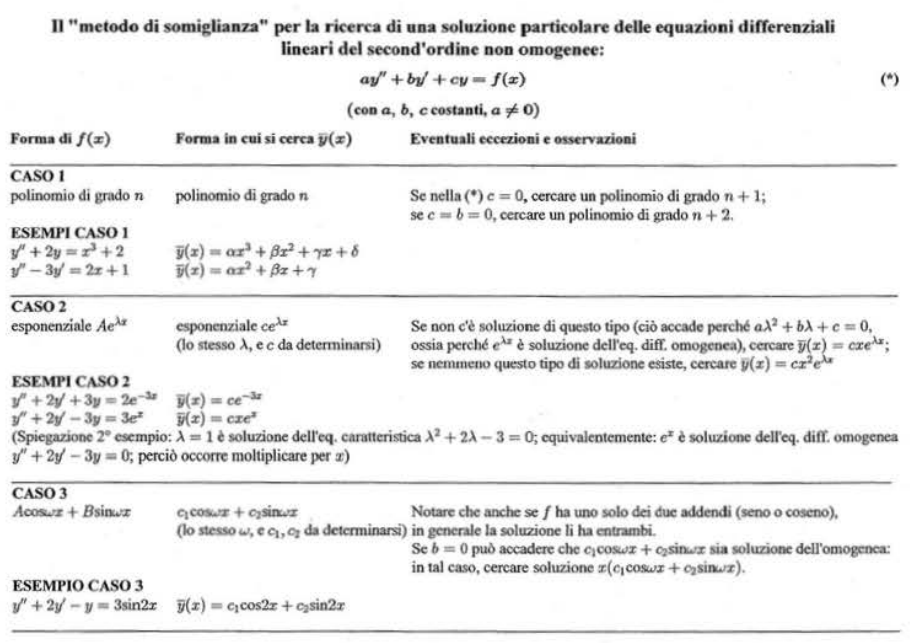
\includegraphics[height=250px]{../img/eqdiff2.PNG}
\end{center}
\begin{center}
    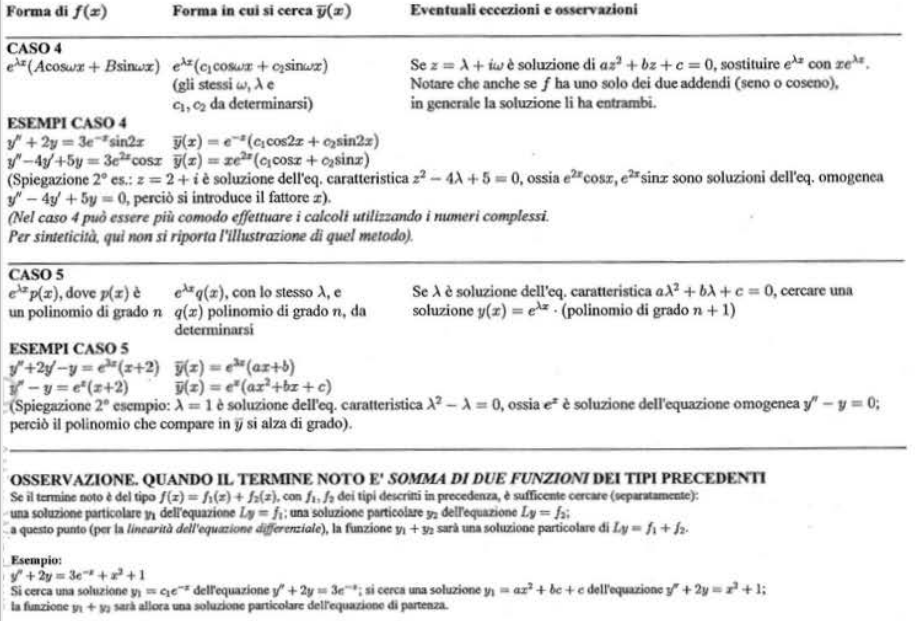
\includegraphics[height=250px]{../img/eqdiff2(1).PNG}
\end{center}